\documentclass[a4paper,twoside]{article}

\usepackage{apalike}
\usepackage{SCITEPRESS}
\usepackage{amssymb}
\usepackage{amstext}
\usepackage{amsmath}
\usepackage{amsthm}
\usepackage{graphicx}
\usepackage{multicol}
\usepackage[small]{caption}
\usepackage{subfloat}

\usepackage{tikz}



\begin{document}


%%%%%%%%%%%%%%%%%%%%%%%%%%%%%%%%%%%%%%%%%%%%%%%%%%%%%%%%%%%%%%%%%%%%%%%%%%%%%%%%
%%%                               80 COLONNES                                %%%
%%%%%%%%%%%%%%%%%%%%%%%%%%%%%%%%%%%%%%%%%%%%%%%%%%%%%%%%%%%%%%%%%%%%%%%%%%%%%%%%


\title{Lessons Learned through Actual Implementation of MAC/RDC Protocols
       on 802.15.4 Radio Medium: the Case of S-CoSenS}


%\author{
%\authorname{K\'evin Roussel, Ye-Qiong Song and Olivier Zendra}
%\affiliation{LORIA/INRIA Nancy Grand-Est,\\
%             Universit\'e de Lorraine,\\
%             615, rue du Jardin Botanique,\\
%             54600 Villers-L\`es-Nancy, France}
%\email{\{Kevin.Roussel,Ye-Qiong.Song,Olivier.Zendra\}@inria.fr}
%}


\keywords{Wireless Sensor Networks, Internet of Things, Heavy Load, QoS,
          MAC/RDC protocols, S-CoSenS, ContikiMAC}


%Nécessité de s'intéresser au cas où les réseaux de WSN ont de fortes charges
%à transmettre, ne serait-ce que ponctuellement ("bursts").

%Std 802.15.4 : délai entre réception d'un paquet et envoi d'un acquittement
%entre deux paquets successifs => rarement respectés.

%Lessons learned during protocol implementations... (Experience report)


\abstract{Implementing new, high-performance MAC/RDC protocols requires
real-time features, to be able to synchronize correctly between different
unrelated devices. Such features are highly desirable for operating wireless
sensor networks (WSN) that are designed to be part of the Internet of Things
(IoT). Unfortunately the operating systems commonly used in this domain
cannot provide such features.\\
In this article, we describe our implementation of a high-performance MAC/RDC
protocol, S-CoSenS, on RIOT OS, a real-time operating system for wireless
sensor networks (WSN) and the Internet of Things (IoT).\\
We then evaluate the performances of our implementation, by comparing it with
the well-known ContikiMAC protocol (running on Contiki OS), through
simulations running on the Cooja emulator. We focus on QoS results,
especially under heavy network loads.\\
Our results show that our protocol performs very well, bringing noticeable
improvements over ContikiMAC results under a large spectrum of network loads
and configurations.}


\onecolumn \maketitle \normalsize \vfill

%%%%%%%%%%%%%%%%%%%%%%%%%%%%%%%%%%%%%%%%%%%%%%%%%%%%%%%%%%%%%%%%%%%%%%%%%%%%%

\section{\uppercase{Introduction}}

TODO.


%%%%%%%%%%%%%%%%%%%%%%%%%%%%%%%%%%%%%%%%%%%%%%%%%%%%%%%%%%%%%%%%%%%%%%%%%%%%%

\section{\uppercase{WSN Software platforms}}

Specialized OSes for the resource-constrained devices that constitute
wireless sensor networks have been designed, published, and made available
for quite a long time.


The current reference OS in the domain of WSN and IoT is \emph{Contiki}
\cite{ContikiOS}. It's also an open-source OS, which was first released
in 2002. It is also at the origin of many assets: we can mention, among
others, the uIP Embedded TCP/IP Stack \cite{uip}, that has been extended
to uIPv6, the low-power Rime network stack \cite{Rime}, or the Cooja
advanced network simulator \cite{Cooja}.

Contiki is very lightweight and well adapted to motes and
resource-constrained devices. It is coded in standard C language, which
makes it relatively easy to learn and program. It offers an event-based
kernel, implemented using cooperative multithreading, and a complete
network stack. All of these features and advantages have made
Contiki widespread, making it the reference OS when it comes to WSN.

Contiki developers also have made advances in the MAC/RDC domain: many
of them have been implemented as part of the Contiki network stack, and
a specifically developed, ContikiMAC, has been published in 2011
\cite{ContikiMAC} and implemented into Contiki as the default
RDC protocol (designed to be used with standard CSMA/CA as MAC layer).

Consequently, we naturally decided, as a comparison reference our first tests,
to use the Contiki software platform: the ContikiOS, the ContikiMAC RDC
protocol, the standard CSMA/CA MAC layer, and the Rime network layer, used
on the IEEE 802.15.4 physical wireless/radio protocol.

\bigskip

However, the Contiki OS also has some limitations that prevented us from
using it as our software platform.

Contiki OS is indeed not a real-time OS: the processing of ``events''---using
Contiki's terminology---is made by using the kernel's scheduler, which is
based on cooperative multitasking. This scheduler only triggers at a specific,
pre-determined rate; on the platforms we're interested in, this rate is
fixed to 128~Hz: this corresponds to a time skew of up to 8~milliseconds
(8000~microseconds) to process an event, interruption management being
one of the possible events. Such a large granularity is clearly
a huge problem when implementing high-performance MAC/RDC protocols,
knowing that the transmission of a full-length 802.15.4 packet takes
bout 4~milliseconds (4000~microseconds), a time granularity of
320~microseconds is needed, corresponding to one backoff period (BP).

In an attempt to address this problem, Contiki provides a real-time feature,
\texttt{rtimer}, which allows to bypass the kernel scheduler and use
a hardware timer to trigger execution of user-defined functions. However,
only one instance of \texttt{rtimer} is available, thus only one
real-time event can be scheduled or executed at any time; this limitation
forbids development of advanced real-time software---like high-performance
MAC~/ RDC protocols---or at least makes it very hard.
Moreover, it is unsafe to execute from \texttt{rtimer}, even
indirectly, most of the Contiki basic functions (i.e.: kernel, network
stack, etc.), because these functions are not designed to handle pre-emption.
Contiki is indeed based on cooperative multithreading, whereas the
\texttt{rtimer} mechanism seems like a ``independent feature'', coming
with its own paradigm.
Only a precise set of functions known as ``interrupt-safe'' (like
\texttt{process\_poll()}) can be safely invoked from \texttt{rtimer},
using other parts of Contiki's meaning almost certainly crash or
unpredictable behaviour. This restriction practically makes it very
difficult to write Contiki extensions (like network stack layer drivers)
using \texttt{rtimer}.

For all these reasons, we were unable to use Contiki OS to develop and
implement our high-performance MAC/RDC protocols. We definitely needed
an OS with efficient real-time features and event handling mechanism.

\bigskip

Consequently, we focused our interest on \emph{RIOT OS} \cite{RIOT}.

This new system---first released in 2013---is also open-source and
specialized in the domain of low-power, embedded wireless sensors.
It offers many interesting features, that we will now describe.

It provides the basic benefits of an OS: portability (it has been ported
to many devices powered by ARM, MSP430, and---more recently---AVR
microcontrollers) and a comprehensive set of features, including
a network stack.

Moreover, it offers key features that are otherwise yet unknown in
the WSN/IoT domain:

\begin{itemize}

\item an efficient, interrupt-driven, tickless \emph{micro-kernel};

\item that kernel includes a priority-aware task scheduler, providing
      \emph{pre-emptive multitasking};

\item a highly efficient use of \emph{hardware timers}: all of them can be
      used concurrently (especially since the kernel is tickless), offering
      the ability to schedule actions with high granularity; on low-end
      devices, based on MSP430 architecture, events can be scheduled
      with a resolution of 32~microseconds;

\item RIOT is entirely written in \emph{standard C language}; but unlike
      Contiki, there are no restrictions on usable constructs (i.e.: like
      those introduced by the protothreads mechanism);

\item a clean and \emph{modular design}, that makes development with and
      \emph{into} the system itself easier and more productive.

\end{itemize}

The first three features listed hereabove make RIOT a full-fledged
\emph{real-time} operating system.

RIOT is a powerful real-time operating system, adapted to the limitations
of deeply embedded hardware microcontrollers, while offering state-of-the-art
techniques (preemptive multitasking, tickless scheduler, optimal use
of hardware timers) that---we believe---makes it on par with
the best OSes of the embedded and real-time world.


%%%%%%%%%%%%%%%%%%%%%%%%%%%%%%%%%%%%%%%%%%%%%%%%%%%%%%%%%%%%%%%%%%%%%%%%%%%%%

\section{\uppercase{Protocols}}
\label{SectProtoDescription}

\subsection{The ContikiMAC RDC protocol}

It is currently the default RDC protocol proposed by the Contiki OS, and
thus it has become a \textit{de facto} standard in the WSN community.
This protocol is designed to work under the classical CSMA/CA MAC layer.

It is technically a derivative of the classical X-MAC protocol \cite{XMAC}:
its basic principle, fundamentally asynchronous, is that every node keep
its radio transceiver off as much as possible, only waking it up for short
delay of radio medium listening at a fixed rate (by default, eight times
per second in ContikiMAC). If, during the short amount of time the radio
transceiver is on, data is sensed on the medium, the radio transceiver
is kept on until the whole transmission is done; otherwise, the node
goes back into ``radio silence mode'' to spare energy.
This ability to automatically adapt the duration of transceiver activity
to the live traffic on radio channel is what makes ContikiMAC a
\emph{auto-adaptative} (or \emph{self-adaptative}) protocol.

When a node has to emit a packet, it continuously emits it until the
intended receiver nodes ``wakes up'' its radio transceiver, receives
the transmitted data, and sends back an acknowledgement.

The first specificity of ContikiMAC is that, during transmission, instead
of emitting a specific preamble until the receiver is ready, then sending
it the actual data packet, the data packet is directly emitted by the
sender---it is its own preamble---so that receiver(s) can directly receive
and acknowledge the data packet as soon as its radio is ready.

The second specificity is the presence of an optimization mechanism named
``transmission phase lock'': senders note the time when they receive
acknowledgement from receivers, and according to the known rate of radio
wake-up, deduce the subsequent expected times when these receivers are
supposed to be ready to receive packets. Thus, senders can synchronize
with nodes that have previously received their transmissions, and can
send their next packets at the optimal period to minimize the useless
transmission of packets when the intended receiver is offline.

%%%%%%%%%%%%%%%%%%%%%%%%%%%%%%%%%%%%%%%%%%%%%%%%%%%%%%%%%%%%%%%%%%%%%%%%%%%%%

\subsection{Our first design: the S-CoSenS MAC/RDC protocol}

The first MAC~/ RDC protocol we wanted to implement is S-CoSenS, which
is designed to work on top of the IEEE 802.15.4 physical layer.

It is an evolution of the already published CoSenS protocol \cite{CosensConf}:
it adds to the latter a sleeping period for energy saving.
Thus, the basic principle of S-CoSenS is to delay the forwarding (routing)
of received packets, by dividing the radio duty cycle in three periods:
a sleeping period (SP), a waiting period (WP) where the radio medium
is listened by routers for collecting incoming 802.15.4 packets, and
finally a burst transmission period (TP) for emitting adequately
the packets enqueued during WP.

Note that in contrast to ContikiMAC, S-CoSenS is based on the \emph{receiver
initiated} paradigm, as implemented in the classical RI-MAC protocol
\cite{RIMAC}.

The main advantage of S-CoSenS is its ability to adapt dynamically to the
wireless network throughput at runtime, by calculating for each radio duty
cycle the length of SP and WP, according to the number of retransmitted
packets during previous cycles. It follows a ``sliding average''
algorithm, where WP duration for each duty cycle is computed as:
\begin{displaymath}
\overline{\mathrm{WP}_{n}} = \alpha \cdot \overline{\mathrm{WP}_{n-1}}
                + (1 - \alpha) \cdot \mathrm{WP}_{n-1}
\end{displaymath}
where $\overline{\mathrm{WP}_{n}}$ and $\overline{\mathrm{WP}_{n-1}}$
are respectively the average WP length at $n^{\mathrm{th}}$ and
$(n-1)^{\mathrm{th}}$ cycle, and $\mathrm{WP}_{n-1}$ is the actual
length of the $(n-1)^{\mathrm{th}}$ cycle.

The local synchronization between a S-CoSenS router and the other nodes
of its PAN is done thanks to a beacon packet, that is broadcasted by
the router at the beginning of each duty cycle. This beacon contains the
duration (in microseconds) of the SP and WP for the currently beginning
duty cycle.

The whole S-CoSenS duty cycle workflow for a PAN router is summarized
in figure \ref{FigSCosensDutyCycle} hereafter.

\begin{figure}[!h]
\centering
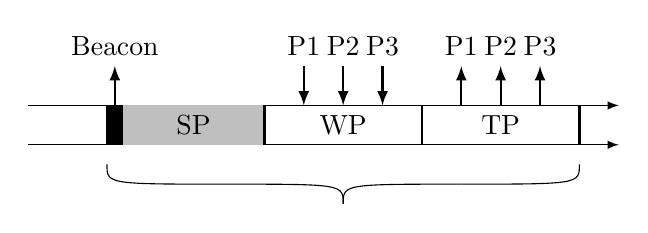
\begin{tikzpicture}[>=latex]
\draw[->] (-1cm,  0.25cm) -- +(7.5cm, 0);
\draw[->] (-1cm, -0.25cm) -- +(7.5cm, 0);
%beacon
\fill[black] (0cm, -0.25cm) rectangle +(0.2cm, 0.5cm);
\draw[->,thick] (0.1cm, 0.25cm) -- +(0, 0.5cm);
\draw (0.1cm, 1cm) node {Beacon};
%SP
\draw[thick] (0cm, -0.25cm) -- +(0, 0.5cm);
\fill[lightgray] (0.2cm, -0.25cm) rectangle +(1.8cm, 0.5cm);
\draw (1.1cm, 0) node {SP};
%WP
\draw[thick] (2cm, -0.25cm) -- +(0, 0.5cm);
\draw (3cm, 0) node {WP};
%TP
\draw[thick] (4cm, -0.25cm) -- +(0, 0.5cm);
\draw (5cm, 0) node {TP};
\draw[thick] (6cm, -0.25cm) -- +(0, 0.5cm);
%RX packets
\draw[->,thick] (2.5cm, 0.75cm) -- +(0, -0.5cm);
\draw (2.5cm, 1cm) node {P1};
\draw[->,thick] (3cm, 0.75cm) -- +(0, -0.5cm);
\draw (3cm, 1cm) node {P2};
\draw[->,thick] (3.5cm, 0.75cm) -- +(0, -0.5cm);
\draw (3.5cm, 1cm) node {P3};
%TX packets
\draw[->,thick] (4.5cm, 0.25cm) -- +(0, 0.5cm);
\draw (4.5cm, 1cm) node {P1};
\draw[->,thick] (5cm, 0.25cm) -- +(0, 0.5cm);
\draw (5cm, 1cm) node {P2};
\draw[->,thick] (5.5cm, 0.25cm) -- +(0, 0.5cm);
\draw (5.5cm, 1cm) node {P3};
%brace
\draw (0cm,-0.5cm)    .. controls +(0,-0.25cm) .. +(1.5cm,-0.25cm);
\draw (1.5cm,-0.75cm) .. controls +(1.5cm,0)   .. +(1.5cm,-0.25cm);
\draw (3cm,-1cm)      .. controls +(0,0.25cm)  .. +(1.5cm,0.25cm);
\draw (4.5cm,-0.75cm) .. controls +(1.5cm,0)   .. +(1.5cm,0.25cm);
\end{tikzpicture}
\caption{A typical S-CoSenS router duty cycle.}
\label{FigSCosensDutyCycle}
\end{figure}

We thus need to synchronize with enough accuracy different devices (that
can be based on different hardware platforms) on duty cycles whose periods
are dynamically calculated at runtime, with resolution that needs to be
in the sub-millisecond range. This is where RIOT OS advanced real-time
features really shine, while the other comparable OSes are
for that purpose definitely lacking.

We have implemented S-CoSenS under RIOT, and evaluated it by comparing
to the ContikiMAC + CSMA/CA couple under Contiki OS.


%%%%%%%%%%%%%%%%%%%%%%%%%%%%%%%%%%%%%%%%%%%%%%%%%%%%%%%%%%%%%%%%%%%%%%%%%%%%%

\section{\uppercase{Method and Benchmark}}

For our first experiments, we used, for practical reasons, the Cooja
simulator rather than actual hardware. All the simulated nodes are
virtual Zolertia Z1 motes, well-known MSP430-based devices, that are
used in real-life, industrial setups.

We have implemented test applications under both Contiki and RIOT OS, and
made first tests by performing simulations of a basic, but large, 802.15.4
PAN (Personal Area Network) constituted of a ``router'', and ten motes
acting as ``leaf nodes''. The ten nodes regularly send data packets to
the router, that retransmits these data packets to a nearby ``sink'' device.
Both the router and the ten nodes use exclusively the S-CoSenS RDC/MAC
protocol. This is summarized in figure \ref{FigPANtest}.

\begin{figure}[!h]
\centering
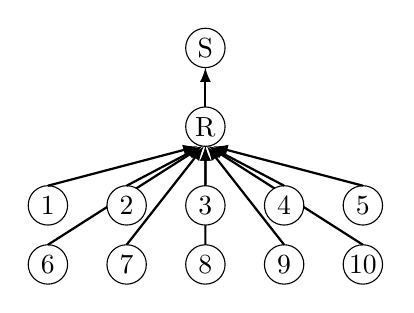
\begin{tikzpicture}[>=latex]
%sink
\draw (0, 1cm) circle (0.25cm); \draw (0, 1cm) node {S};
%router to sink link
\draw[->,thick] (0, 0.25cm) -- (0, 0.75cm);
%router
\draw (0, 0) circle (0.25cm); \draw (0, 0) node {R};
%leaf nodes (lower)
\foreach \x in {6,7,8,9,10}
{
  \fill[white] (\x * 1cm - 8cm, -1.75cm) circle (0.25cm);
  \draw (\x * 1cm - 8cm, -1.75cm) circle (0.25cm);
  \draw (\x * 1cm - 8cm, -1.75cm) node {\x};
  % link to router
  \draw[->,thick] (\x * 1cm - 8cm, -1.5cm)
                  -- (\x * 0.02cm - 0.16cm, -0.25cm);
}
%leaf nodes (upper)
\foreach \x in {1,2,3,4,5}
{
  \fill[white] (\x * 1cm - 3cm, -1cm) circle (0.25cm);
  \draw (\x * 1cm - 3cm, -1cm) circle (0.25cm);
  \draw (\x * 1cm - 3cm, -1cm) node {\x};
  % link to router
  \draw[->,thick] (\x * 1cm - 3cm, -0.75cm)
                  -- (\x * 0.05cm - 0.15cm, -0.25cm);
}
\end{tikzpicture}
\caption{Functional schema of our virtual test PAN.}
\label{FigPANtest}
\end{figure}

We then performed simulations on this virtual PAN, varying several parameters
of the ContikiMAC RDC protocol, under moderately-heavy to extreme network
loads. The loads were generated by the application loaded on the 10 leaf
nodes: they were programmed to generate large 802.15.4 network packets
(90 bytes of payload, which translates to an actual packet size of
around 110 bytes) at a fixed rate, with random variations to avoid
medium congestion. The different setups are described in table
\ref{TblDataRates}: the table gives the average delay between
each packet transmission on each mote, the average number of
packets emitted every second for the 10 nodes, and the expected
resulting data rate.

\begin{table}[htb]
\centering
\begin{tabular}{|l|r|r|r|}
\hline
Setup     &  Delay  & Pkts/s & Data Rate \\
\hline
Moderate  & 1500 ms &   6.7  &  5,867 bit/s \\ 
High      & 1000 ms &  10    &  8,800 bit/s \\
Very High &  500 ms &  20    & 17,600 bit/s \\
Extreme   &  100 ms & 100    & 88,000 bit/s \\
\hline
\end{tabular}
\caption{Transmission data rates used on leaf nodes.}
\label{TblDataRates}
\end{table}

For each scenario, we performed two kind of simulations:
\begin{itemize}
\item a \emph{fixed packet number simulation}, during which each node emits
500 packets at the fixed rate, then turns off; the simulation ends when all
nodes have transmitted their quota of packets;

\item a \emph{fixed duration simulation}, during which each node emits an
unspecified number of packets at the fixed rate; the simulation ends after
10 minutes.
\end{itemize}

These different kind of simulations allow us to easily compute respectively
QoS data and duty cycle statistics, as we will now see in the next section.


%%%%%%%%%%%%%%%%%%%%%%%%%%%%%%%%%%%%%%%%%%%%%%%%%%%%%%%%%%%%%%%%%%%%%%%%%%%%%

\section{\uppercase{Results and Discussion}}

\subsection{Quality of Service (QoS)}

We quantify the QoS, in our simulations of WSN, by the number of packets
that arrive to their destination, that is: the number of packets that are
sent from one of the leaf nodes, relayed by the router, and are actually
received by the sink.

Using the \emph{fixed packet number simulations}, we can easily compute the
rate of packets that arrive to destination, compared to the known number
of packets emitted by the nodes.

Thus, we were able to determine that the only parameter that has actually
influence on the QoS is the length of the duty cycle on S-CoSenS, which
corresponds in the ContikiMAC RDC protocol to the rate at which the radio
medium is sensed (this parameter is named
\texttt{NETSTACK\_CONF\_RDC\_CHANNEL\_CHECK\_RATE} in Contiki source code).
Its default value is 8, meaning the radio channel is checked eight times
per second; this parameter is actually given in Hertz.
In S-CoSenS, the default duration for the subframe is 100 ms.

Note that we also allowed, on Contiki, the the standard CSMA/CA MAC layer
to perform up to seven retries for a given data packet, by setting the
\texttt{CSMA\_CONF\_MAX\_MAC\_TRANSMISSIONS}
parameter to 8 in Contiki source code. This was done in order to put it
on par with S-CoSenS default configuration, where a packet can by default
be transmitted up to 8 times before being cancelled.
Note however, that  the ``retry'' term does not have the same signification
under S-CoSenS---where it specifies the reemission of \emph{one} instance of
a packet---than on ContikiMAC where it specifies a new duty cycle during
which the packet is reemitted an unspecified number of times. This is
the consequence of the fundamental difference in design between the two
protocols (see section \ref{SectProtoDescription} above).

This default value of 8~Hz only gives poor results concerning QoS.
We changed the parameter value, and doubled it up to 256~Hz. The results
we obtained are shown in table \ref{TblSuccessRate}.

\begin{table*}[htbp]
\centering
\begin{tabular}{|r|r|r|r|r|}
\hline
Setup & Moderate & High & Very High & Extreme \\
\hline
\multicolumn{5}{|l|}{Channel Check Rate = 8 Hz}\\
\hline
NODES & & & & \\
packets lost & 121 & 190 & 1086 & 3190 \\
packets transmitted & 4879 & 4810 & 3914 & 1810 \\
success rate & 97.58\% & 96.20\% & 78.28\% & 36.20\% \\
ROUTER & & & & \\
packets lost & 2394 & 3167 & 3194 & 1778 \\
packets transmitted & 2485 & 1641 & 722 & 32 \\
success rate & 49.70\% & 32.82\% & 14.44\% & 0.64\% \\
\hline
\multicolumn{5}{|l|}{Channel Check Rate = 16 Hz}\\
\hline
NODES & & & & \\
packets lost & 14 & 48 & 173 & 2532 \\
packets transmitted & 4986 & 4952 & 4827 & 2468 \\
success rate & 99.72\% & 99.04\% & 96.54\% & 49.36\% \\
ROUTER & & & & \\
packets lost & 39 & 1029 & 3724 & 2042 \\
packets transmitted & 4947 & 3922 & 1106 & 434 \\
success rate & 98.94\% & 78.44\% & 22.12\% & 8.68\% \\
\hline
\multicolumn{5}{|l|}{Channel Check Rate = 32 Hz}\\
\hline
NODES & & & & \\
packets lost & 0 & 3 & 41 & 1668 \\
packets transmitted & 5000 & 4997 & 4959 & 3332 \\
success rate & 100\% & 99.94\% & 99.18\% & 66.64\% \\
ROUTER & & & & \\
packets lost & 0 & 0 & 641 & 3048 \\
packets transmitted & 5000 & 4996 & 4316 & 299 \\
success rate & 100\% & 99.92\% & 86.32\% & 5.98\% \\
\hline
Setup & Moderate & High & Very High & Extreme \\
\hline
\end{tabular}
\caption{Rate of packets arrived to their destination,
         according to the ContikiMAC channel check rate.\\
         Results obtained with fixed packet number simulations.}
\label{TblSuccessRate}
\end{table*}

The data shown in table \ref{TblSuccessRate} shows us many facts:

\begin{itemize}

\item ContikiMAC QoS increases with Channel Check Rate.

\item S-CoSenS QoS results are significantly better than ConikiMAC's,
      and are much more stable when the duty cycle duration changes.

\item With ContikiMAC, the packet losses are mainly due to the router.

\item With S-CoSens, the router never loses the packets it receives:
      all losses occur between leaf nodes and router.

\end{itemize}

%%%%%%%%%%%%%%%%%%%%%%%%%%%%%%%%%%%%%%%%%%%%%%%%%%%%%%%%%%%%%%%%%%%%%%%%%%%%%

\subsection{Delays}

TODO

%%%%%%%%%%%%%%%%%%%%%%%%%%%%%%%%%%%%%%%%%%%%%%%%%%%%%%%%%%%%%%%%%%%%%%%%%%%%%

\subsection{Limitations and Inconsistencies}
\label{SectLimits}

The current work has of course its limitations:

\begin{itemize}

\item \emph{Those are only simulations.} To be truly accurate, we would need
to run these tests on actual hardware.\\
Moreover, we constated, during our simulations, an anomaly in the MSPSim
software (the MSP430 device simulator used by Cooja to emulate MSP430-based
motes at the cycle level \cite{MSPSim}): \emph{the delay used by the
simulator to load our large---around 110 bytes---IEEE 802.15.4 packets into
the CC2420 transceiver TX buffer is too long;} it takes around 3~milliseconds
to load such a packet to the transceiver in simulation, while our tests
on the real Zolertia Z1 hardware have explicitely and undoubtly shown that
loading times are actually about 1~millisecond long. We didn't have time
to investigate the problem and correct that anomaly.\\
We also don't know whether or not there are other inconsistencies in
the simulator software that could also alter the results of our
simulations...\\
Such anomalies will probably change the results obtained on real
hardware using the same scenarii and parameters. Unfortunately, we don't
have enough Z1 motes nor time to perform these real-life tests yet.

\item \emph{We didn't have time to study other results.} We especially
didn't have time to study radio traces to determine the transmission
delay of packets from leaf nodes up to their destination (sink).

\end{itemize}

However, we firmly believe that the general facts we observed in our
simulations won't be overturned by these problems. That's why we still
present them in the current article.


%%%%%%%%%%%%%%%%%%%%%%%%%%%%%%%%%%%%%%%%%%%%%%%%%%%%%%%%%%%%%%%%%%%%%%%%%%%%%

\section{\uppercase{Conclusion and Future Works}}

We have build simulation scenarios to test whether our MAC/RDC protocol,
ContikiMAC, could handle heavy network loads, trying to approach the
theoretical limit of 250~kbit/s of bandwith for the underlying
IEEE 802.15.4 radio medium.

We were able to show---with the limits and preventions discussed hereabove
in section \ref{SectLimits}---that it performs quite well under these
situations, and does it better than the reference software platform, in terms
of QoS and packet transmission delays: it can handle quite gracefully some of
the heavy loads we imposed on it during our simulations, managing to obtain
a good to excellent QoS---that is: few packets lost during transmissions.
(Under extreme loads however, it becomes impossible to obtain satisfactory
results for QoS: the radio medium becoming saturated causes the MAC/RDC
layer to stall and become ineffective.)

One must also accept that there is no way to keep the very low power
consumption feature when dealing with such heavy network loads, the
motes' radio transceivers being heavily activated and solicited to
handle that charge.

\medskip

In the future, we would like to try other software platforms with the same
scenarii, especially by using different MAC and RDC layers in the network
stacks, and different operating systems. We may also try to use different,
new hardware devices to run our tests.

We hope to find a way to get a similar or better QoS than the one we observed
here, while trying to optimize duty cycle statistics to minimize the energy
consumption when running WSN under heavy network loads.


%%%%%%%%%%%%%%%%%%%%%%%%%%%%%%%%%%%%%%%%%%%%%%%%%%%%%%%%%%%%%%%%%%%%%%%%%%%%%


\vfill
\bibliographystyle{apalike}
{\small
\bibliography{wowmom2015}}


\end{document}
